\documentclass[14pt]{extbook}
\usepackage{multicol, enumerate, enumitem, hyperref, color, soul, setspace, parskip, fancyhdr} %General Packages
\usepackage{amssymb, amsthm, amsmath, bbm, latexsym, units, mathtools} %Math Packages
\everymath{\displaystyle} %All math in Display Style
% Packages with additional options
\usepackage[headsep=0.5cm,headheight=12pt, left=1 in,right= 1 in,top= 1 in,bottom= 1 in]{geometry}
\usepackage[usenames,dvipsnames]{xcolor}
\usepackage{dashrule}  % Package to use the command below to create lines between items
\newcommand{\litem}[1]{\item#1\hspace*{-1cm}\rule{\textwidth}{0.4pt}}
\pagestyle{fancy}
\lhead{Makeup Progress Quiz -1}
\chead{}
\rhead{Version C}
\lfoot{7547-2949}
\cfoot{}
\rfoot{Fall 2020}
\begin{document}

\begin{enumerate}
\litem{
Solve the rational equation below. Then, choose the interval(s) that the solution(s) belongs to.\[ \frac{9}{2x + 8} + -7 = \frac{2}{-14x -56} \]\begin{enumerate}[label=\Alph*.]
\item \( x_1 \in [-3.36, -3.31] \text{ and } x_2 \in [4.66,6.66] \)
\item \( x \in [-3.34,-2.34] \)
\item \( x \in [4.61,4.69] \)
\item \( x_1 \in [-3.54, -3.39] \text{ and } x_2 \in [-4.34,-1.34] \)
\item \( \text{All solutions lead to invalid or complex values in the equation.} \)

\end{enumerate} }
\litem{
Choose the graph of the equation below.\[ f(x) = \frac{-1}{(x - 1)^2} + 3 \]\begin{enumerate}[label=\Alph*.]
\begin{multicols}{2}\item 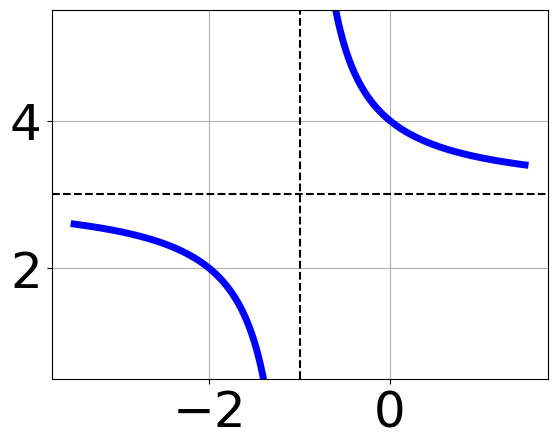
\includegraphics[width = 0.3\textwidth]{../Figures/rationalEquationToGraphCopyAC.png}\item 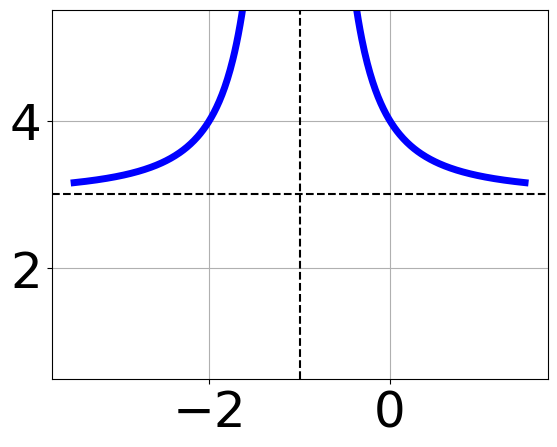
\includegraphics[width = 0.3\textwidth]{../Figures/rationalEquationToGraphCopyBC.png}\item 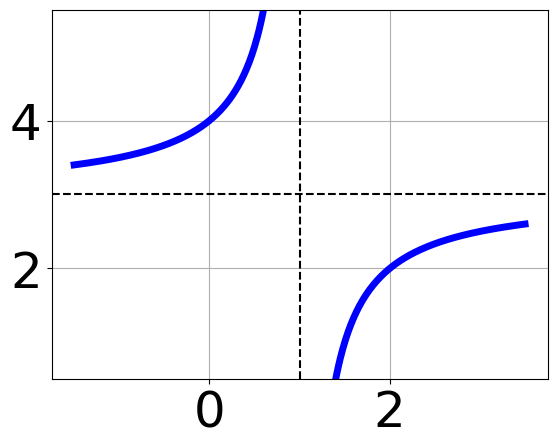
\includegraphics[width = 0.3\textwidth]{../Figures/rationalEquationToGraphCopyCC.png}\item 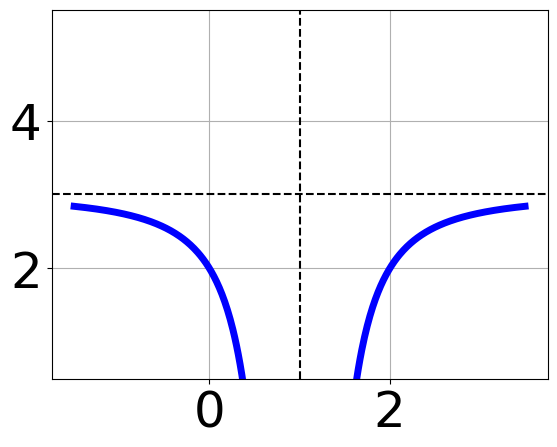
\includegraphics[width = 0.3\textwidth]{../Figures/rationalEquationToGraphCopyDC.png}\end{multicols}\item None of the above.
\end{enumerate} }
\litem{
Solve the rational equation below. Then, choose the interval(s) that the solution(s) belongs to.\[ \frac{-54}{63x -36} + 1 = \frac{-54}{63x -36} \]\begin{enumerate}[label=\Alph*.]
\item \( x_1 \in [-0.2, 2] \text{ and } x_2 \in [0.57,1.57] \)
\item \( \text{All solutions lead to invalid or complex values in the equation.} \)
\item \( x \in [-0.43,1.57] \)
\item \( x \in [-1.7,0.3] \)
\item \( x_1 \in [-1.7, 0.3] \text{ and } x_2 \in [0.57,1.57] \)

\end{enumerate} }
\litem{
Determine the domain of the function below.\[ f(x) = \frac{5}{20x^{2} +5 x -25} \]\begin{enumerate}[label=\Alph*.]
\item \( \text{All Real numbers except } x = a \text{ and } x = b, \text{ where } a \in [-1.25, 0.75] \text{ and } b \in [-1, 3] \)
\item \( \text{All Real numbers.} \)
\item \( \text{All Real numbers except } x = a, \text{ where } a \in [-1.25, 0.75] \)
\item \( \text{All Real numbers except } x = a, \text{ where } a \in [-23, -17] \)
\item \( \text{All Real numbers except } x = a \text{ and } x = b, \text{ where } a \in [-23, -17] \text{ and } b \in [22, 29] \)

\end{enumerate} }
\litem{
Choose the equation of the function graphed below.
\begin{center}
    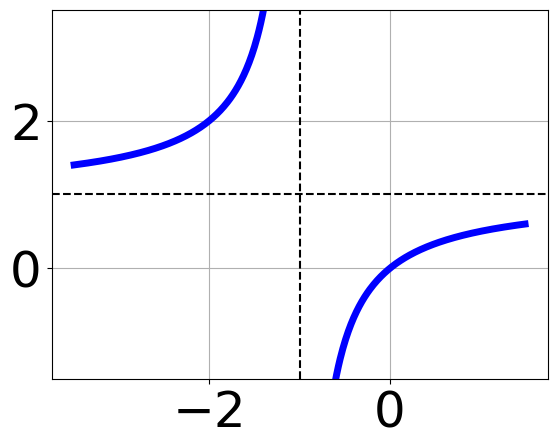
\includegraphics[width=0.5\textwidth]{../Figures/rationalGraphToEquationCopyC.png}
\end{center}
\begin{enumerate}[label=\Alph*.]
\item \( f(x) = \frac{1}{x - 1} + 1 \)
\item \( f(x) = \frac{1}{(x - 1)^2} + 1 \)
\item \( f(x) = \frac{-1}{x + 1} + 1 \)
\item \( f(x) = \frac{-1}{(x + 1)^2} + 1 \)
\item \( \text{None of the above} \)

\end{enumerate} }
\litem{
Determine the domain of the function below.\[ f(x) = \frac{5}{24x^{2} +38 x + 15} \]\begin{enumerate}[label=\Alph*.]
\item \( \text{All Real numbers except } x = a, \text{ where } a \in [-30.08, -29.77] \)
\item \( \text{All Real numbers except } x = a \text{ and } x = b, \text{ where } a \in [-1.17, -0.82] \text{ and } b \in [-0.76, -0.48] \)
\item \( \text{All Real numbers except } x = a, \text{ where } a \in [-1.17, -0.82] \)
\item \( \text{All Real numbers except } x = a \text{ and } x = b, \text{ where } a \in [-30.08, -29.77] \text{ and } b \in [-12.01, -11.79] \)
\item \( \text{All Real numbers.} \)

\end{enumerate} }
\litem{
Choose the equation of the function graphed below.
\begin{center}
    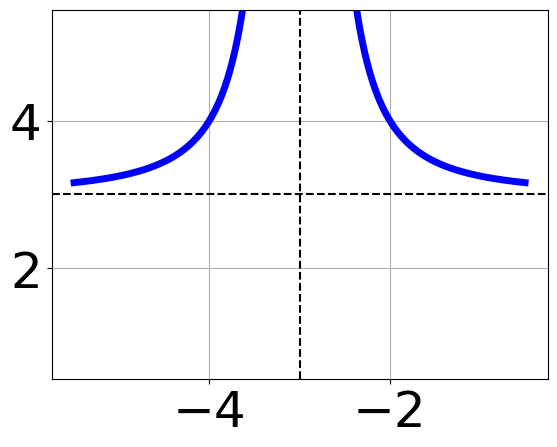
\includegraphics[width=0.5\textwidth]{../Figures/rationalGraphToEquationC.png}
\end{center}
\begin{enumerate}[label=\Alph*.]
\item \( f(x) = \frac{1}{x - 3} - 1 \)
\item \( f(x) = \frac{1}{(x - 3)^2} - 1 \)
\item \( f(x) = \frac{-1}{x + 3} - 1 \)
\item \( f(x) = \frac{-1}{(x + 3)^2} - 1 \)
\item \( \text{None of the above} \)

\end{enumerate} }
\litem{
Solve the rational equation below. Then, choose the interval(s) that the solution(s) belongs to.\[ \frac{-5x}{7x -5} + \frac{-4x^{2}}{35x^{2} -11 x -10} = \frac{2}{5x + 2} \]\begin{enumerate}[label=\Alph*.]
\item \( x_1 \in [0.01, 0.8] \text{ and } x_2 \in [-0.92,0.86] \)
\item \( x_1 \in [0.01, 0.8] \text{ and } x_2 \in [-2.7,0.17] \)
\item \( x \in [-1.92,-0.76] \)
\item \( \text{All solutions lead to invalid or complex values in the equation.} \)
\item \( x \in [-0.95,0.08] \)

\end{enumerate} }
\litem{
Choose the graph of the equation below.\[ f(x) = \frac{-1}{x + 1} - 1 \]\begin{enumerate}[label=\Alph*.]
\begin{multicols}{2}\item 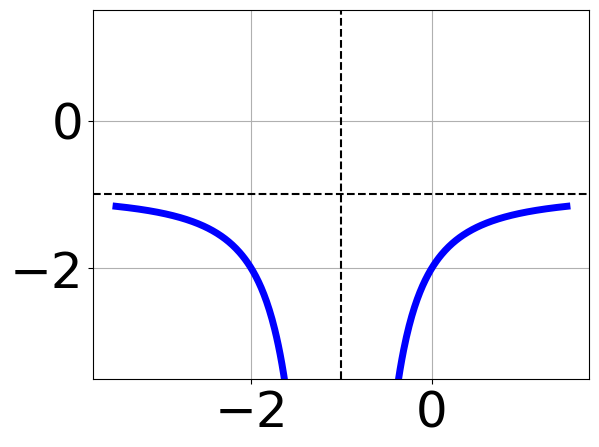
\includegraphics[width = 0.3\textwidth]{../Figures/rationalEquationToGraphAC.png}\item 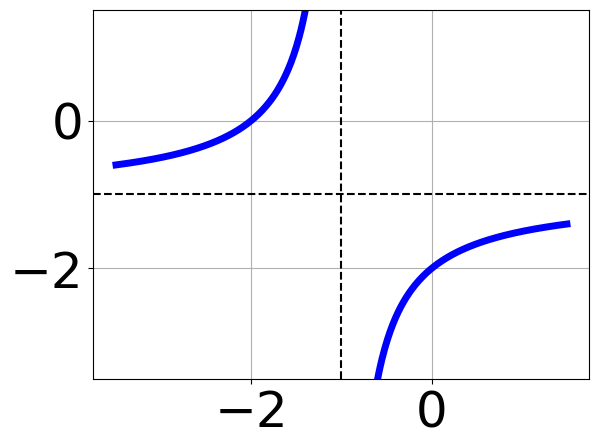
\includegraphics[width = 0.3\textwidth]{../Figures/rationalEquationToGraphBC.png}\item 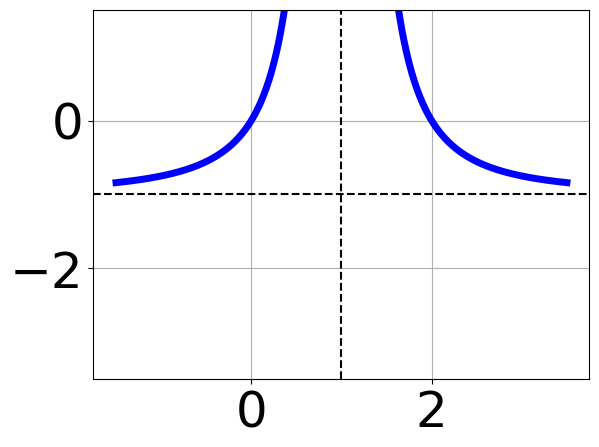
\includegraphics[width = 0.3\textwidth]{../Figures/rationalEquationToGraphCC.png}\item 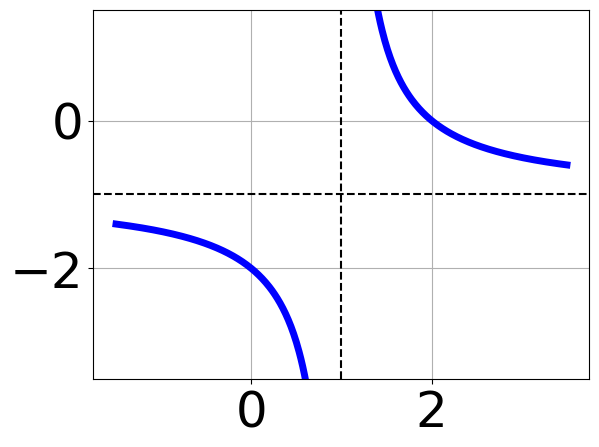
\includegraphics[width = 0.3\textwidth]{../Figures/rationalEquationToGraphDC.png}\end{multicols}\item None of the above.
\end{enumerate} }
\litem{
Solve the rational equation below. Then, choose the interval(s) that the solution(s) belongs to.\[ \frac{7x}{-2x -3} + \frac{-2x^{2}}{-8x^{2} -6 x + 9} = \frac{-3}{4x -3} \]\begin{enumerate}[label=\Alph*.]
\item \( x_1 \in [-0.48, -0.11] \text{ and } x_2 \in [1.3,2.3] \)
\item \( x \in [0.23,1.2] \)
\item \( \text{All solutions lead to invalid or complex values in the equation.} \)
\item \( x \in [1.09,1.92] \)
\item \( x_1 \in [-0.48, -0.11] \text{ and } x_2 \in [-2.5,0.5] \)

\end{enumerate} }
\end{enumerate}

\end{document}